



% \KOMAoptions{paper=a4}

% \recalctypearea


%   \vspace*{\fill}
%   \begin{figure}[H]
%     \centering
%       \includegraphics[width=0.8\textwidth]{#1}
%     \caption{#2}
%     \label{fig:#3}
%   \end{figure}
%   \vspace*{\fill}


% \eject \pdfpagewidth=420mm \pdfpageheight=297mm
% \let\oldhsize\hsize
% \let\hsize2\oldhsize
% \begin{landscape}
 
\KOMAoptions{paper=a1,paper=landscape}
\recalctypearea
 \chapter{Complete Petri Net} 


  \begin{figure}[h]
    \centering
    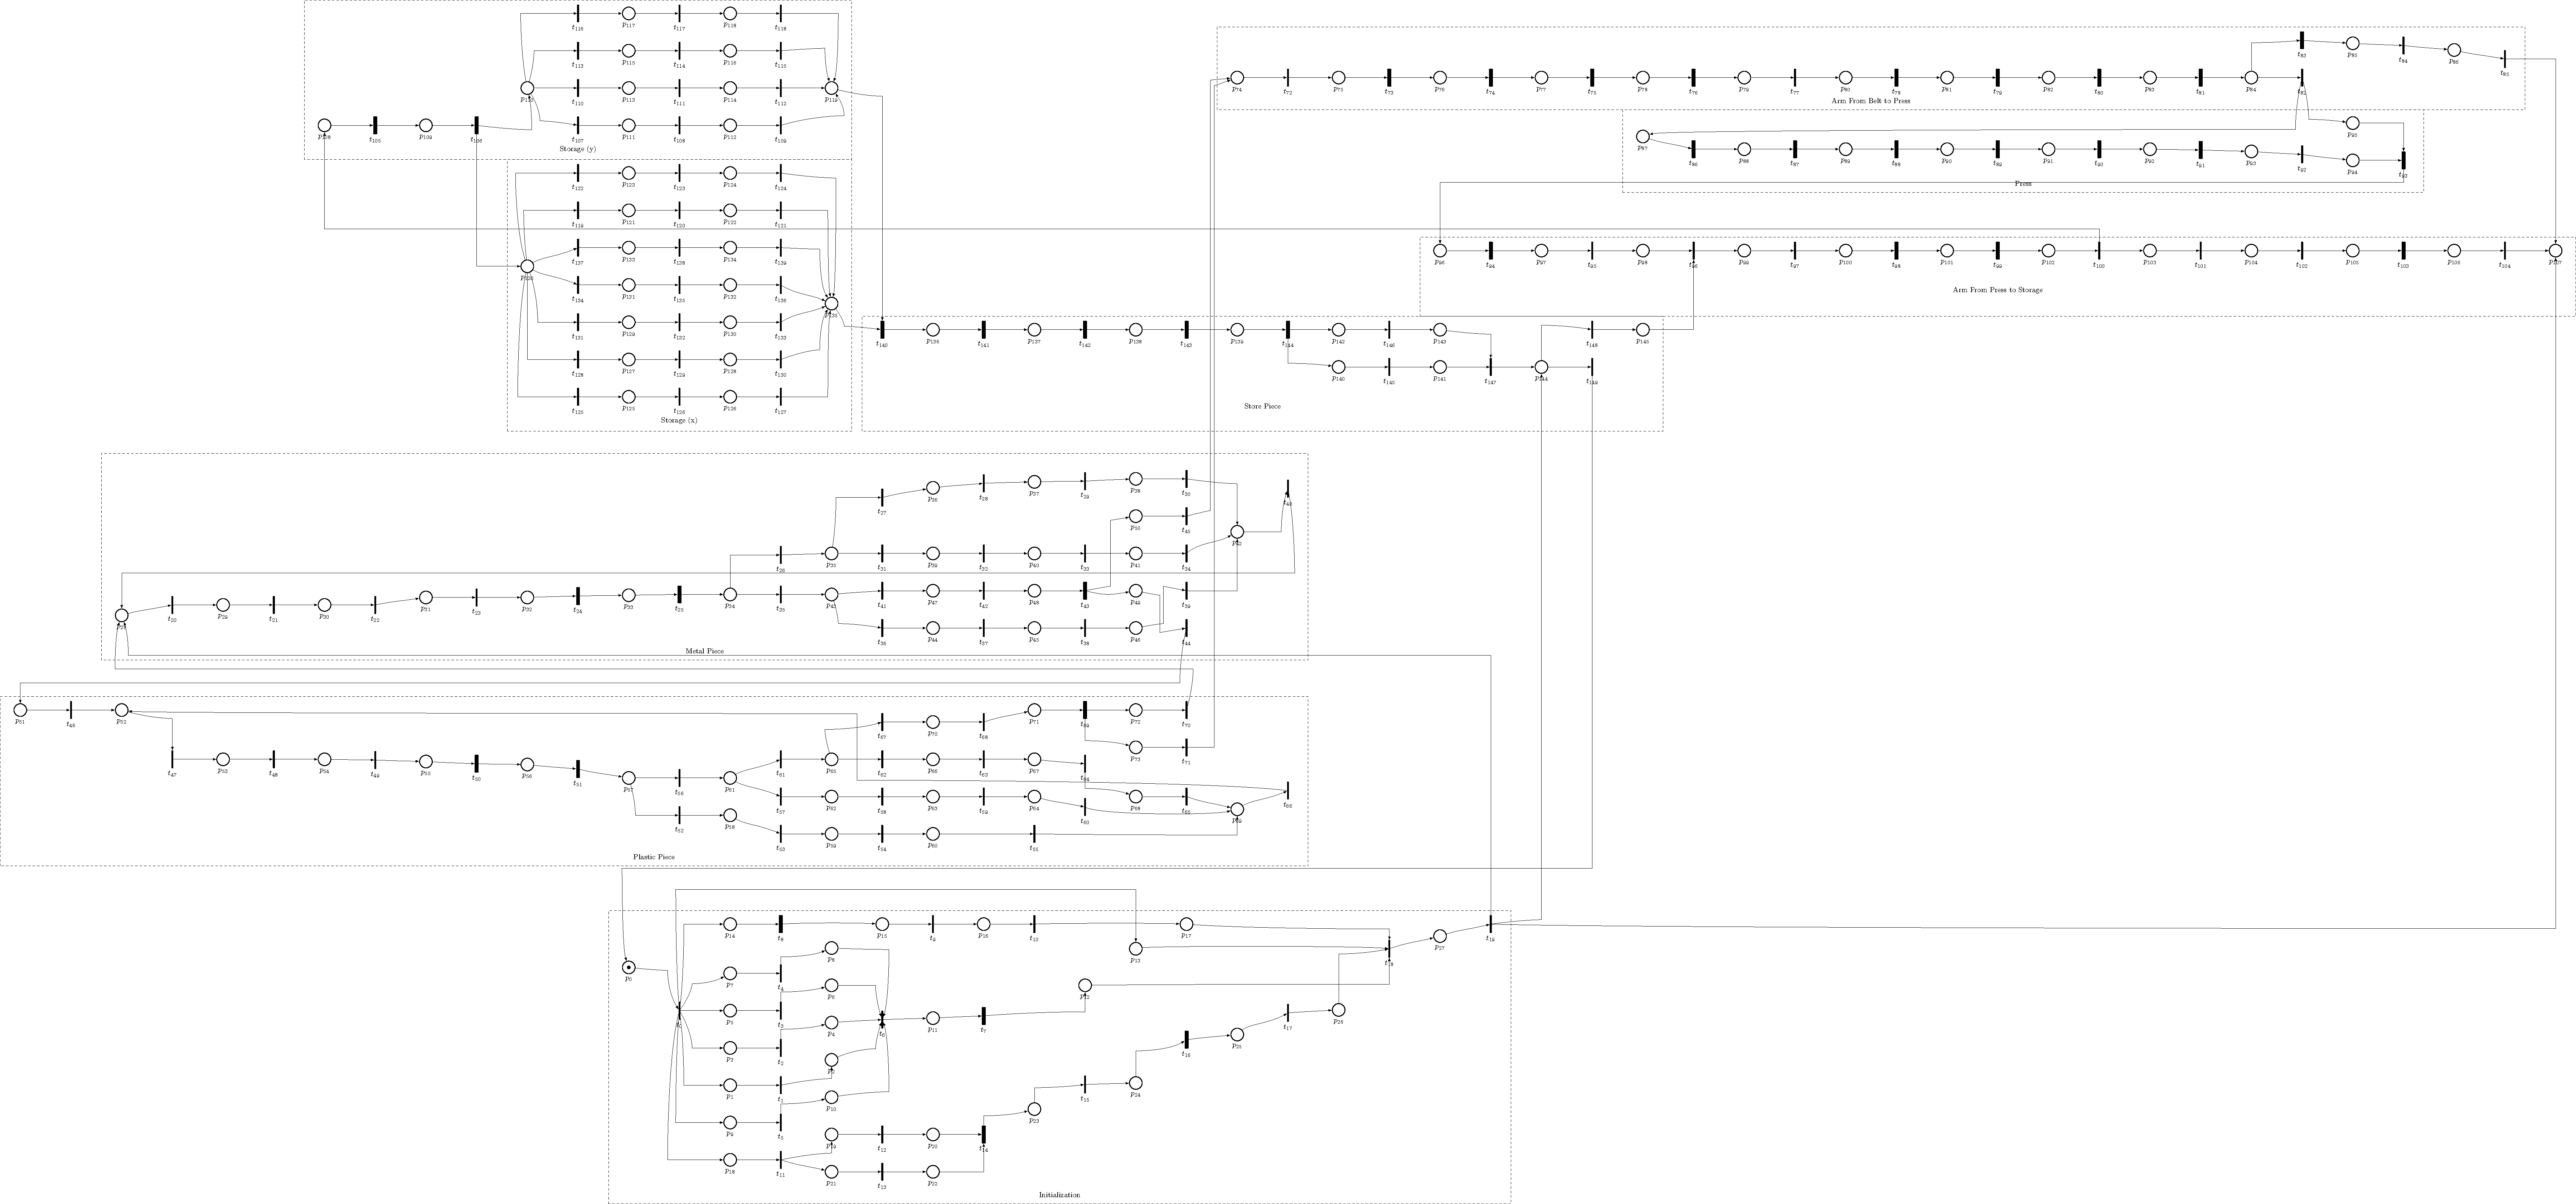
\includegraphics[width=0.8\textwidth]{../../figures/petriNets/dot/completo/completo.pdf}
  \end{figure}

  % \end{landscape}
% \eject \pdfpagewidth=210mm \pdfpageheight=297mm
% \KOMAoptions{paper=a4}
% \recalctypearea
\KOMAoptions{paper=a4,paper=portrait}
\recalctypearea

%%% Local Variables:
%%% mode: latex
%%% TeX-master: "../monografia"
%%% End:
